\chapter{Anhang}

\section{UI-Demos}
\begin{figure}[!htbp]
	\centering
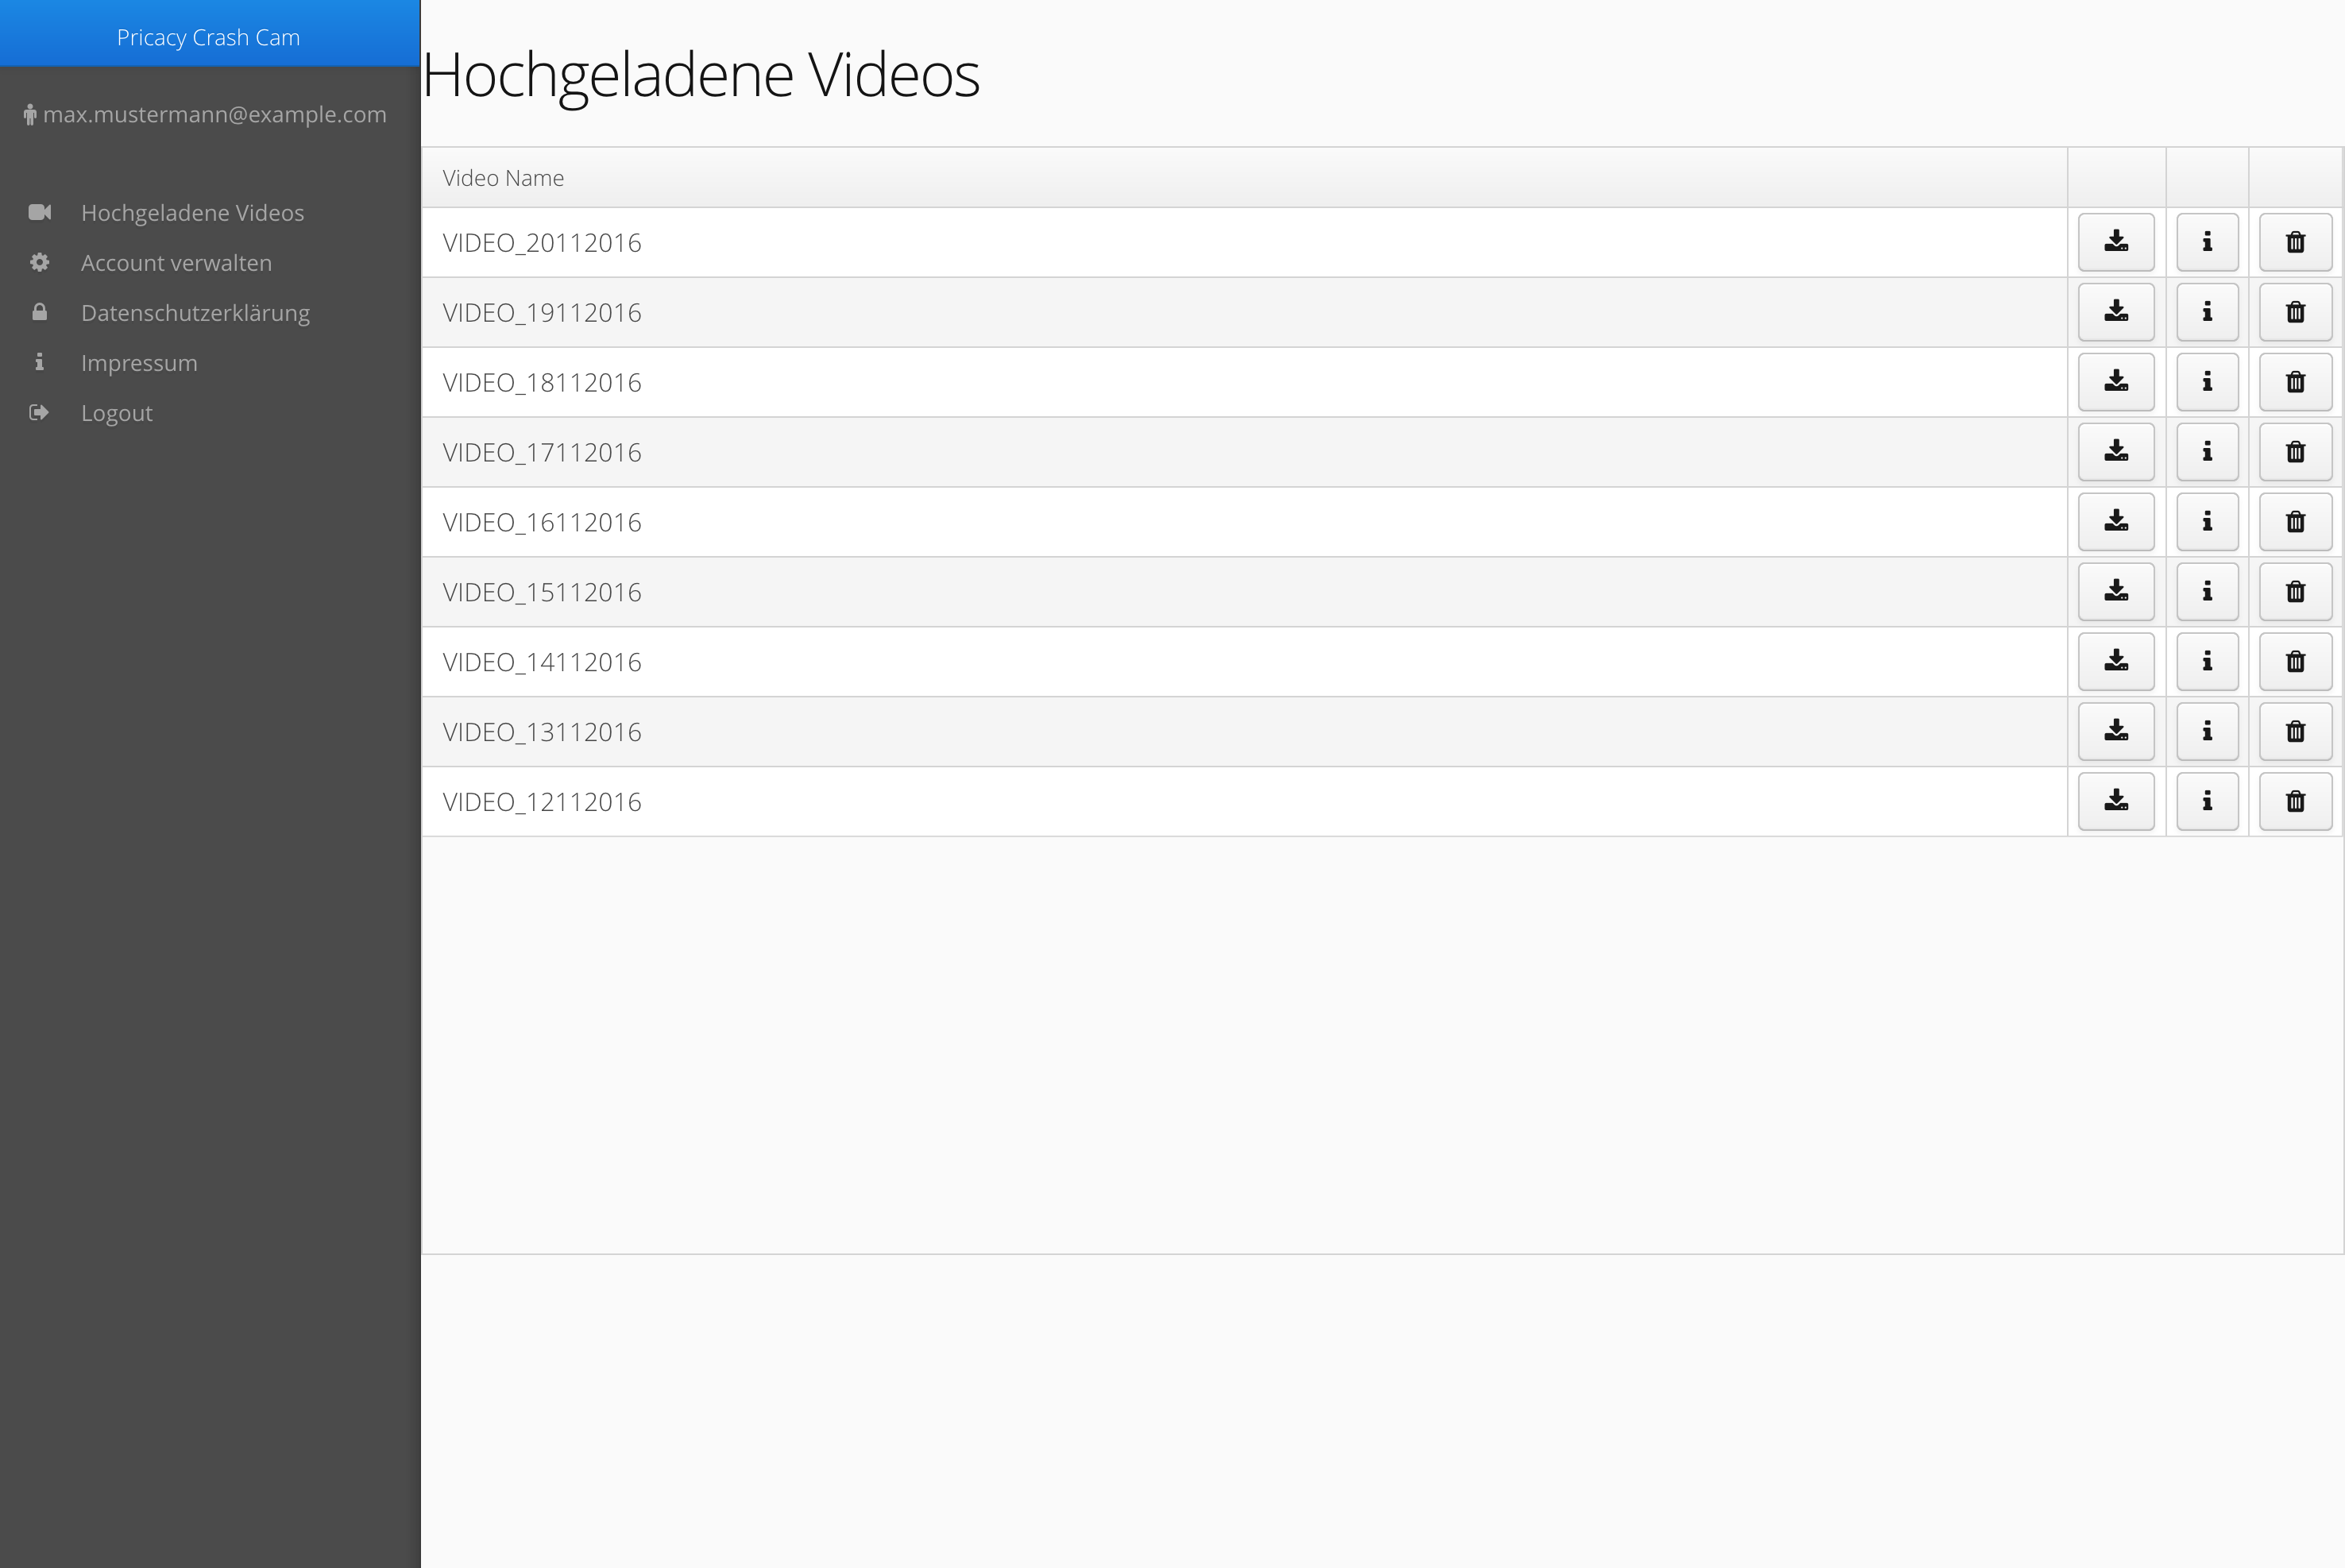
\includegraphics[width=1\textwidth]{subtopicsFuncspec/Res/UI-Demos/Webinterface.png}
	\caption{Web-Interface}
\end{figure}
\begin{figure}
	\centering
	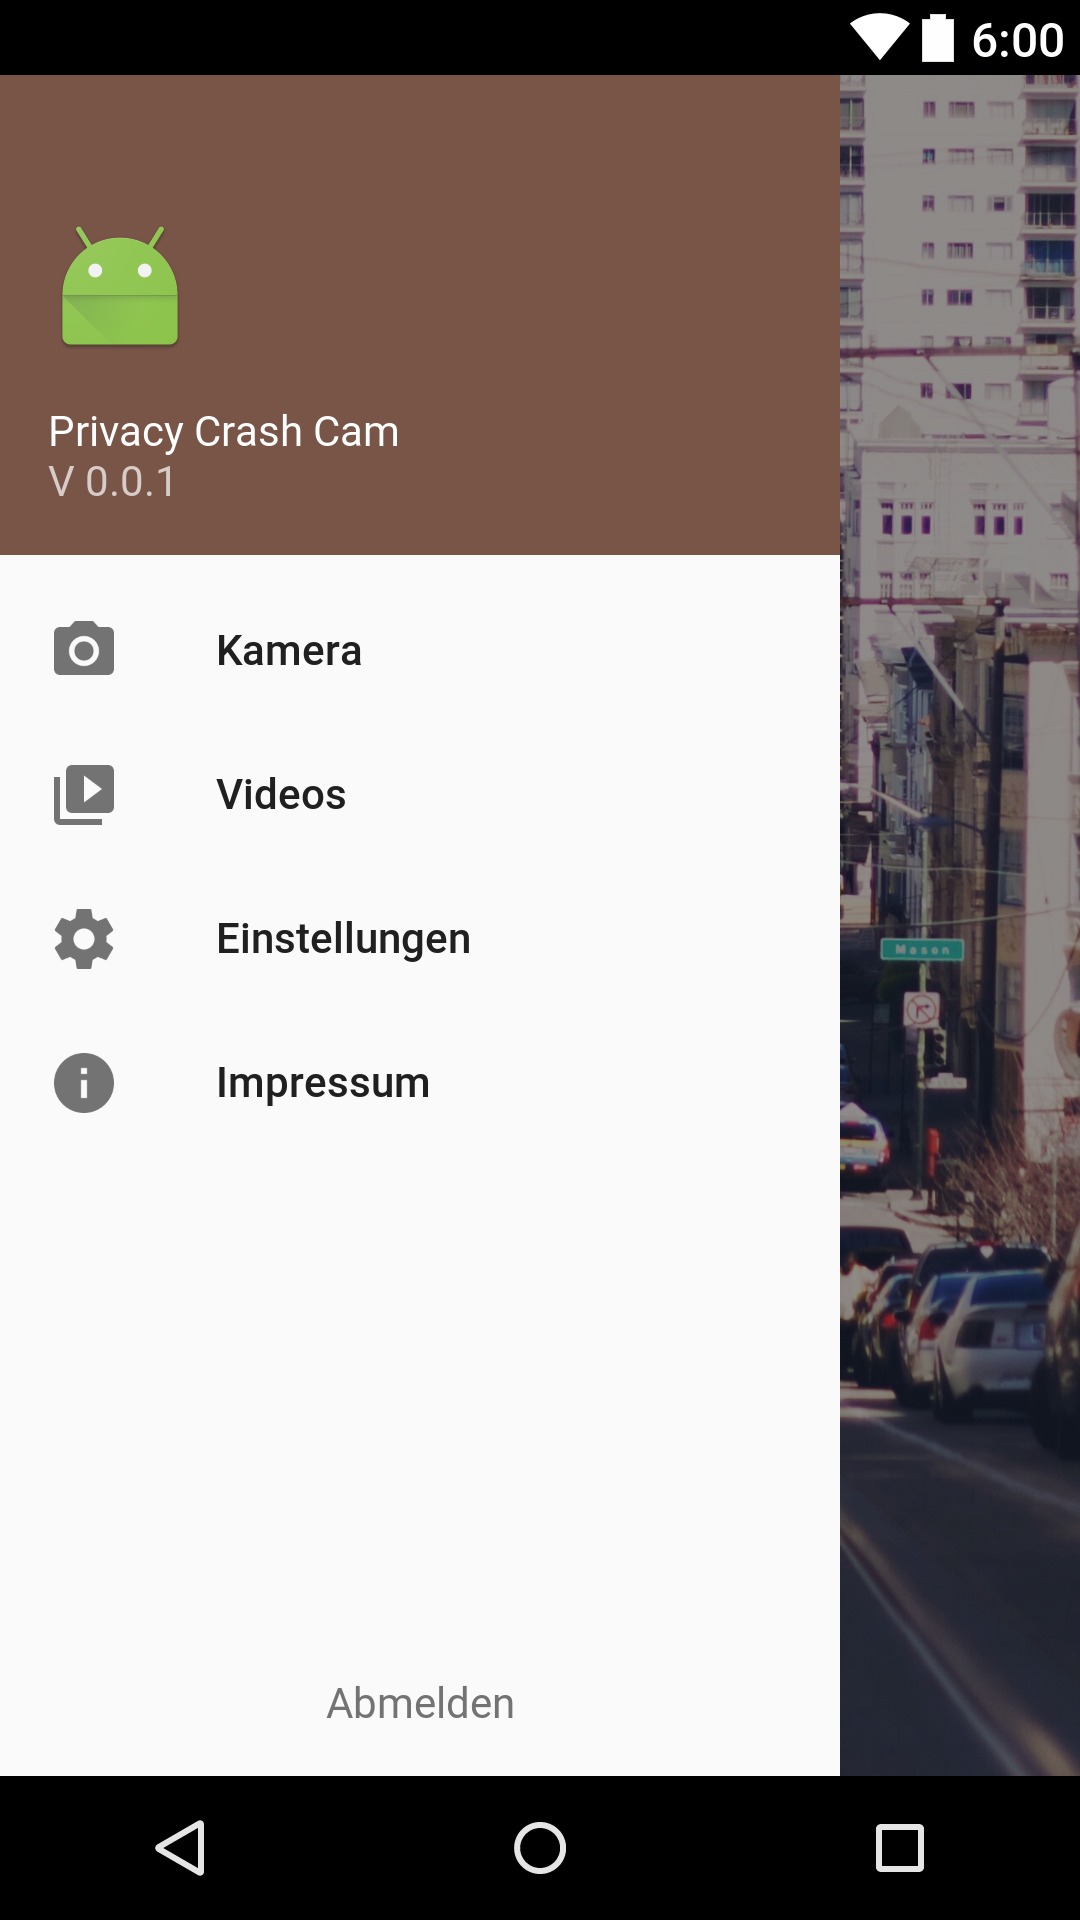
\includegraphics[width=0.33\textwidth]{subtopicsFuncspec/Res/Mockups/Portrait_camera_view_menu.png}
	\caption{Menü}
\end{figure}
\begin{figure}
	\centering
	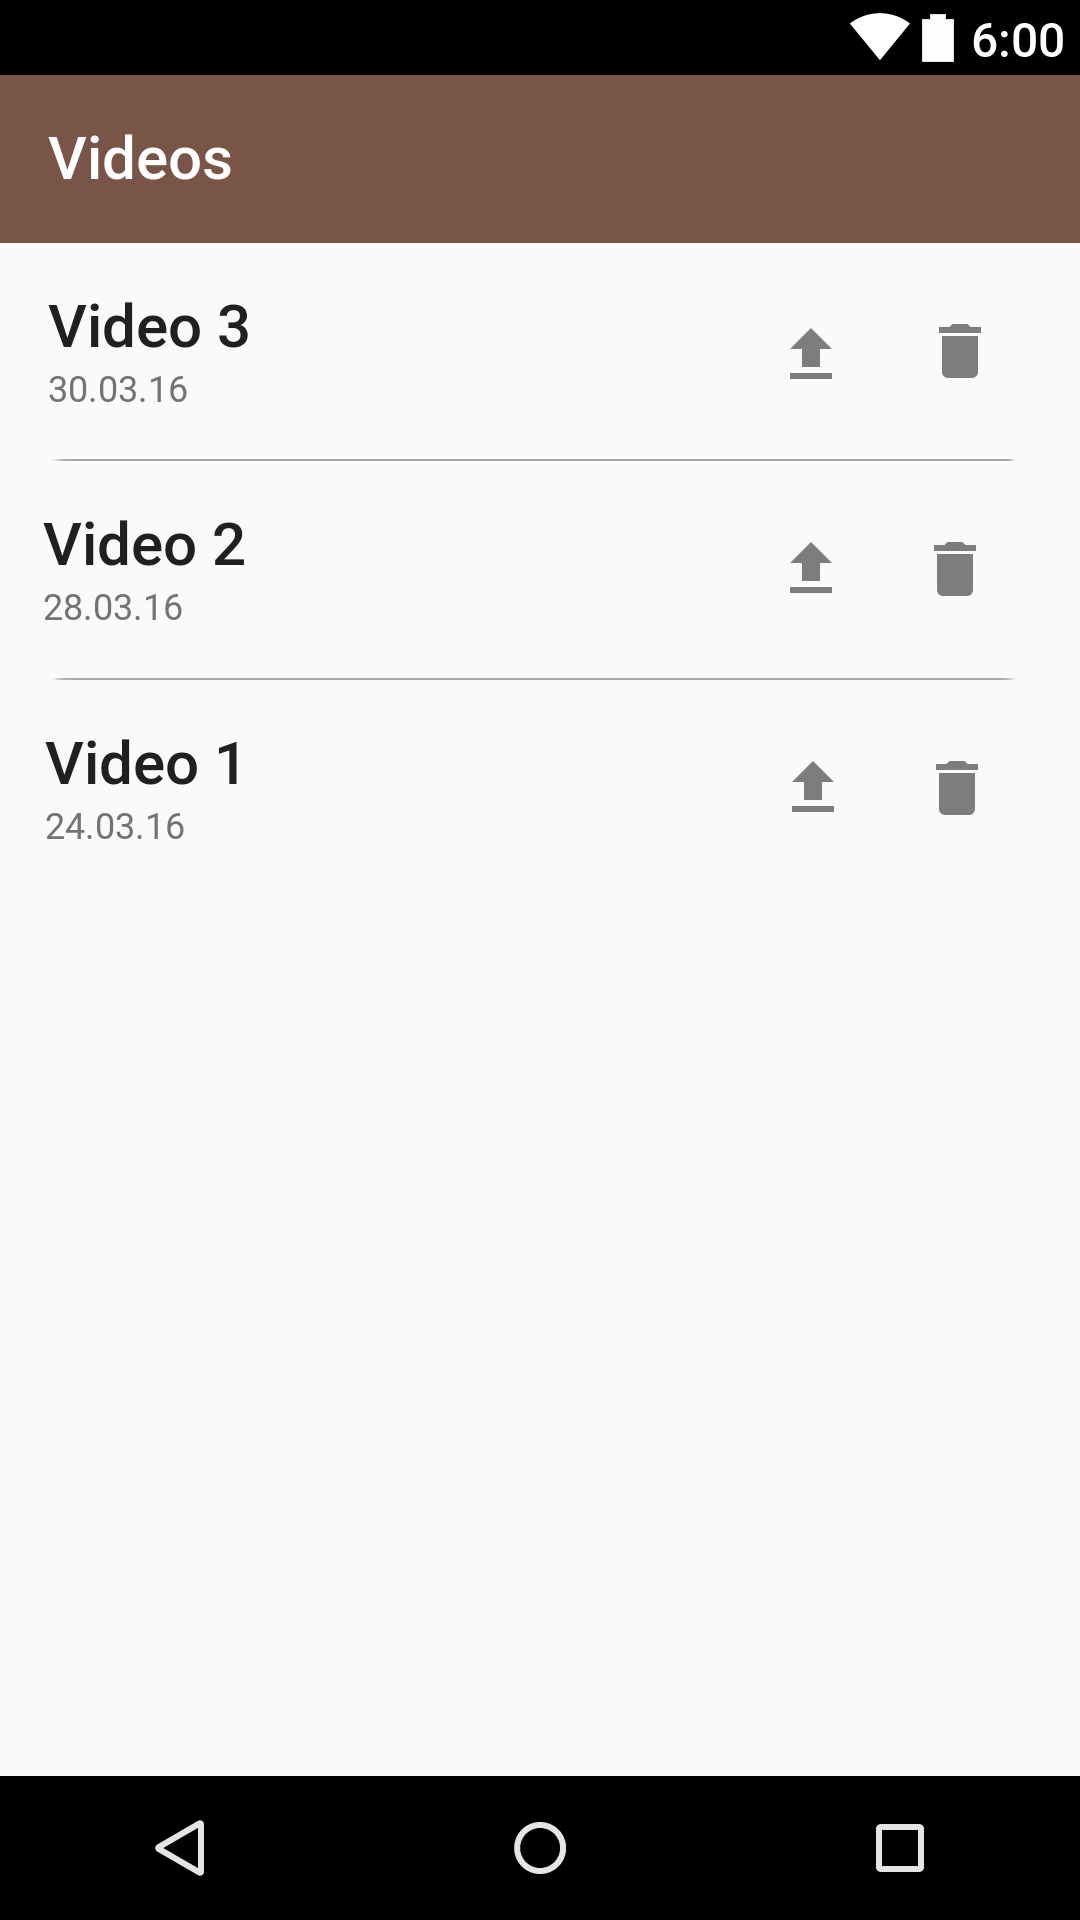
\includegraphics[width=0.33\textwidth]{subtopicsFuncspec/Res/Mockups/Videos_list1.png}
	\caption{Videos}
\end{figure}
\begin{figure}
	\centering
	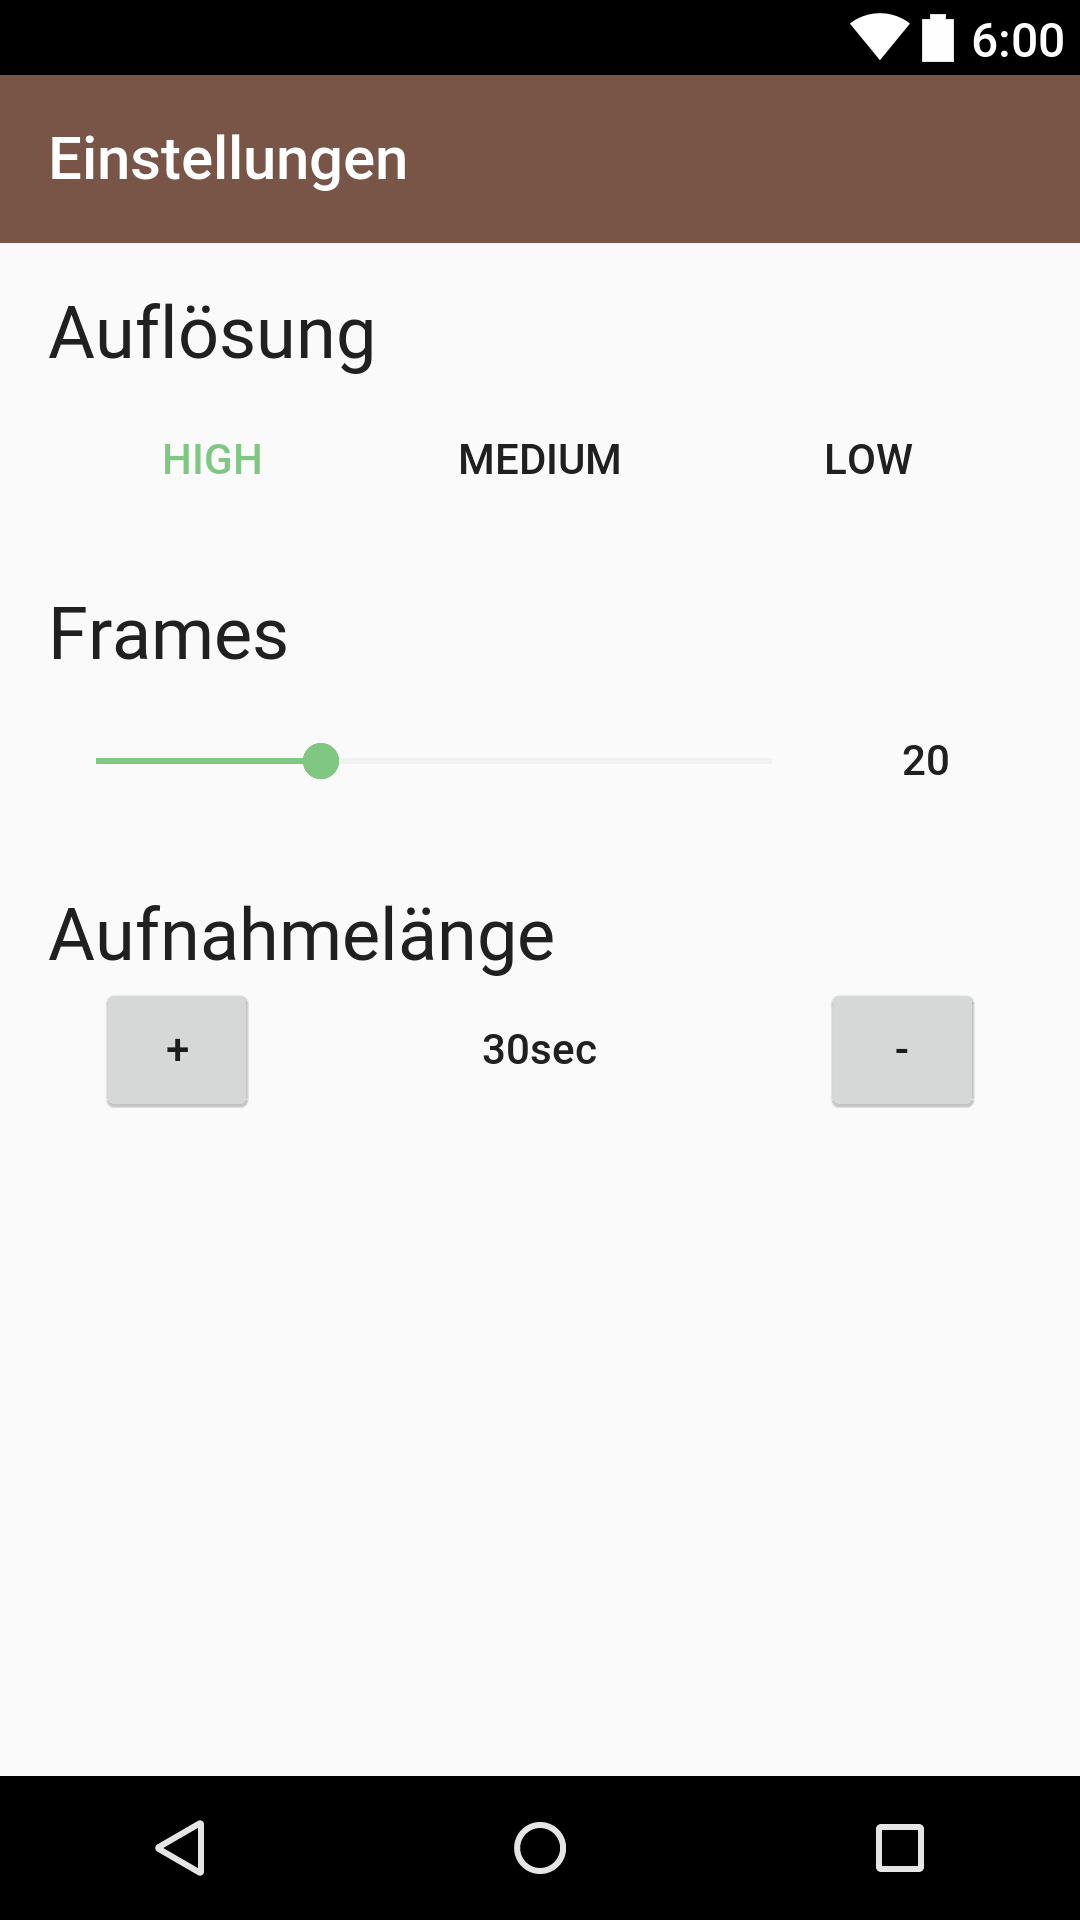
\includegraphics[width=0.33\textwidth]{subtopicsFuncspec/Res/Mockups/Settings1.png}
 	 \caption{Einstellungen}
\end{figure}

\newpage

\section{Verschlüsselung} \label{sec:Verschlüsselung}

Um den Datenschutz zu gewährleisten, ist die Verschl\"usselung eine zentrale Funktion der App und des Web-Dienst. Hierbei m\"ussen die Videos vor der Anonymisierung verschlüsselt gespeichert werden. Dabei wendet die App beim Persistieren eine hybride Verschlüsselung an. Die hybdride Verschlüsselung verbindet dabei die Geschwindigkeit von symmetrischer Verschlüsselung mit der Sicherheit asymetrsicher Verschlüsselung.\\
Zunächst wählt die App einen zufälligen symmetrischen Schlüssel. Mit diesem Schlüssel wird das Video symmetrisch verschlüsselt. Anschließend wird der Schlüssel asymmetrisch mit dem öffentlichen Schlüssel des Web-Dienst verschlüsselt. \\
Als kryptographisches Verfahren werden hierbei AES für die symmetrische und RSA für die asymetrische Verschlüsselung verwendet.


\newpage
\printglossaries
\newglossaryentry{Android}
{
  name = Android,
  description = {Android ist ein von Open Handset Alliance entwickletes Betriebssystem, sowie eine Software Platform für mobile Geräte(\gls{Smartphone} und \gls{Tablet}). Dabei handelt es sich um eine freie und quelloffene Software, die auf einem Linux-Kernel basiert},
}
\newglossaryentry{App}
{
  name = App,
  plural = Apps,
  description = {Als Applikationen, oder eher als Kurzform App bekannt, wird eine Anwendungssoftware auf einem Betriebssystem bezeichnet. Bei mobilen Applikationen wird zwischen verschiedenen Typen unterschieden. Zum einen existieren native Apps (Platformabhängig), Web-, und Cross-Plattform-Apps (Platformunabhängig)},
}
\newglossaryentry{IDE}
{
	name = IDE,
	plural = IDEs,
	description = {Eine IDE (integrierte Entwicklungsumgebung) ist eine Sammlung von Programmen zur Softwareentwicklung},
}
\newglossaryentry{API}
{
  name = API,
  description = {Eine API (Application Programming Interface), auf deutsch Programmierschnittstelle genannt, macht es einfacher ein Programm zu entwickeln, indem sie vorgefertigte Funktionen zur Verfügung stellt. Diese werden mit einem Softwaresystem mitgeliefert und stellen eine Programmieranbindung auf Quelltext-Ebene dar},
}
\newglossaryentry{Web-Dienst}
{
  name = Web-Dienst,
  plural = Web-Dienste,
  description = {Web-Dienste (auch Web-Service) sind Softwareanwendungen, die über ein Netzwerk bereitgestellt werden},
}
\newglossaryentry{Web-Interface}
{
  name = Web-Interface,
  plural = Web-Interfaces,
  description = {Ein Web-Interface (auch Web-Schnittstelle), bezeichnet eine\linebreak Schnittstelle zu einem System, die über ein Netzwerk angesprochen wird. Dabei wird unterschieden zwischen einer grafischen Benutzerobfläche und einem \gls{Web-Dienst}, durch das mit einem anderen System interagiert werden kann},
}
\newglossaryentry{G-Sensor}
{
  name = G-Sensor,
  plural = G-Sensoren,
  description = {Der G-Sensor (bekannt als Beschleunigungssensor), ist ein Sensor der die Beschleunigung in verschiedene Bewegungsrichtungen misst},
}
\newglossaryentry{Metadaten}
{
  name = Metadaten,
  description = {Metadaten enthalten Informationen über andere Dateien. Diese Informationen werden bei der Ansammlung größerer Datenmengen (wie Dokumente, Datenbanken oder Dateien) benötigt, um diese zu verwalten},
}
\newglossaryentry{persistieren}
{
  name = persistieren,
  description = {Die Persistierung (Verb: persistieren) wird in der Informatik häufig als ``nicht flüchtige Datenspeicherung'' definert. Dadurch wird die Funktion, Daten oder Objekte über längere Zeit zu speichern, beschrieben},
}
\newglossaryentry{anonymisieren}
{
  name = anonymisieren,
  description = {Mit Anonymisierung bezeichnet man den Vorgang, personenbezogene Daten so zu ändern, dass diese Daten nicht mehr einer Person zugeordnet werden können},
}
\newglossaryentry{E-Mail}
{
  name = E-Mail,
  plural = E-Mails,
  description = {Ein E-Mail ist eine briefähnliche Nachricht, die zwischen Personen mit bestimmten Netzwerkverbindungen auf einem definierten System verschickt werden kann},
}
\newglossaryentry{Smartphone}
{
  name = Smartphone,
  plural = Smartphones,
  description = {Ein Smartphone ist ein Mobilfunkgerät, das die Funktionalität eines herkömmlichen Mobiltelefons überschreitet und diese mit umfangreicheren Computer-Funktionalitäten erweitert},
}
\newglossaryentry{Push-Benachrichtigung}
{
  name = Push-Benachrichtigung,
  plural = Push-Benachrichtigungen,
  description = {Push-Benachrichtigungen sind Meldungen, die ohne das Öffnen der jeweiligen \gls{App} auf dem \gls{Smartphone} erscheinen},
}
\newglossaryentry{Livestream}
{
  name = Livestream,
  plural = Livestreams,
  description = {Ein Livestream (auf deutsch Echtzeitübertragung), ist das Öffnen eines digitale Übertragungskanals. Über diesen kann ein Datenstrom, bestehend aus Video- und Audiomaterial in Echtzeit verschickt und empfangen werden},
}
\newglossaryentry{Tablet}
{
  name = Tablet,
  plural = Tablets,
  description = {Tablets (auch bekannt als Tablet-PC), sind flache, tragbare Computer. Sie besitzen meist die gleichen Standartfunktionen wie ein normaler PC (möglicher Anschluss von Maus und Tastatur, WLAN), aber auch Funktionen eines \gls{Smartphone} (Multitouchscreen oder Bedienung per Stift)},
}
\newglossaryentry{iOS}
{
  name = iOS,
  description = {iOS ist ein von Apple entwickelte mobiles Betriebssystem für deren hergestellte Mobilgeräte, wie das iPhone},
}
\newglossaryentry{Windows Phone}
{
  name = Windows Phone,
  description = {Windows Phone ist ein Betriebssystem für Smartphones, das von Microsoft entwickelt wurde},
}
\newglossaryentry{Ringpuffer}
{
  name = Ringpuffer,
  description = {Der Ringpuffer (oder auch in der Informatik als Warteschlange bekannt) ist eine Datenstruktur, bei der diejenigen Elemente, die zuerst gespeichert wurden, auch zuerst wieder aus dem Speicher entnommen werden, wenn dieser vollläuft},
}
\newglossaryentry{RSA}
{
  name = RSA,
  description = {RSA ist ein populäres asymmetrisches kryptographisches Verfahren, das auf dem Faktorisierungsproblem beruht},
}
\newglossaryentry{Kryptografisches Verfahren}
{
  name = Kryptografisches Verfahren,
  description = {Unter Kryptografie versteht man die Lehre von Geheimschriften. Kryptographische Verfahren werden dazu verwendet Dateien zu Verschlüsseln und diese somit vor nicht autorisierten Lesern zu schützen},
}
\newglossaryentry{Responsive-Design}
{
  name = Responsive-Design,
  description = {Responsive Webdesign bezeichnet die Gestaltung von Oberflächen in der Form, dass diese sich an die Eigenschaften des Endgeräts anpassen},
}
\newglossaryentry{AES}
{
  name = AES,
  description = {AES (Advanced Encryption Standard), ist ein standardisiertes symmetrisches Verschlüsselungsverfahren, das auf Blockverschlüsselung beruht},
}
\newglossaryentry{Java-Servlet}
{
  name = Java-Servlet,
  plural = Java-Servlets,
  description = {Als Java-Servlets bezeichnet man Klassen in Java, die Fähigkeiten eines Webservers erweitern, indem sie Anfragen von Clients beantworten und entgegennehmen. Dabei ist die Besonderheit die dynamische Antworterstellung, die je nach Anfrage variiert},
}
\newglossaryentry{Hash-Code}
{
  name = Hash-Code,
  description = {Hashing ist eine Funktion, die aus einem Klartext beliebiger Länge eine Zeichenkette fester Länge, den Hash-Code, erstellt. Dabei ist es nicht direkt möglich aus dem Hash-Code auf die ursprüngliche Zeichenkette zu schließen},
}

